\lecture{Представление, визуализация и использование изображений}{Анна Ермолович}

\subsection{Введение}
Следует понимать, что все изображения, которые может видеть человеческий глаз, всегда плоские. Человек не умеет видеть трехмерные изображения. Из-за этого почти никогда нет необходимости в полном трехмерном воспроизведении. Соответственно, возникает вопрос, как визуализировать некоторые геометрические объекты на плоскости. Например, как может визуализировать монитор. Существует два классических подхода, как мы можем что-то визуализировать: \textbf{растровые изображения}, \textbf{векторные изображения}.
\begin{center}
    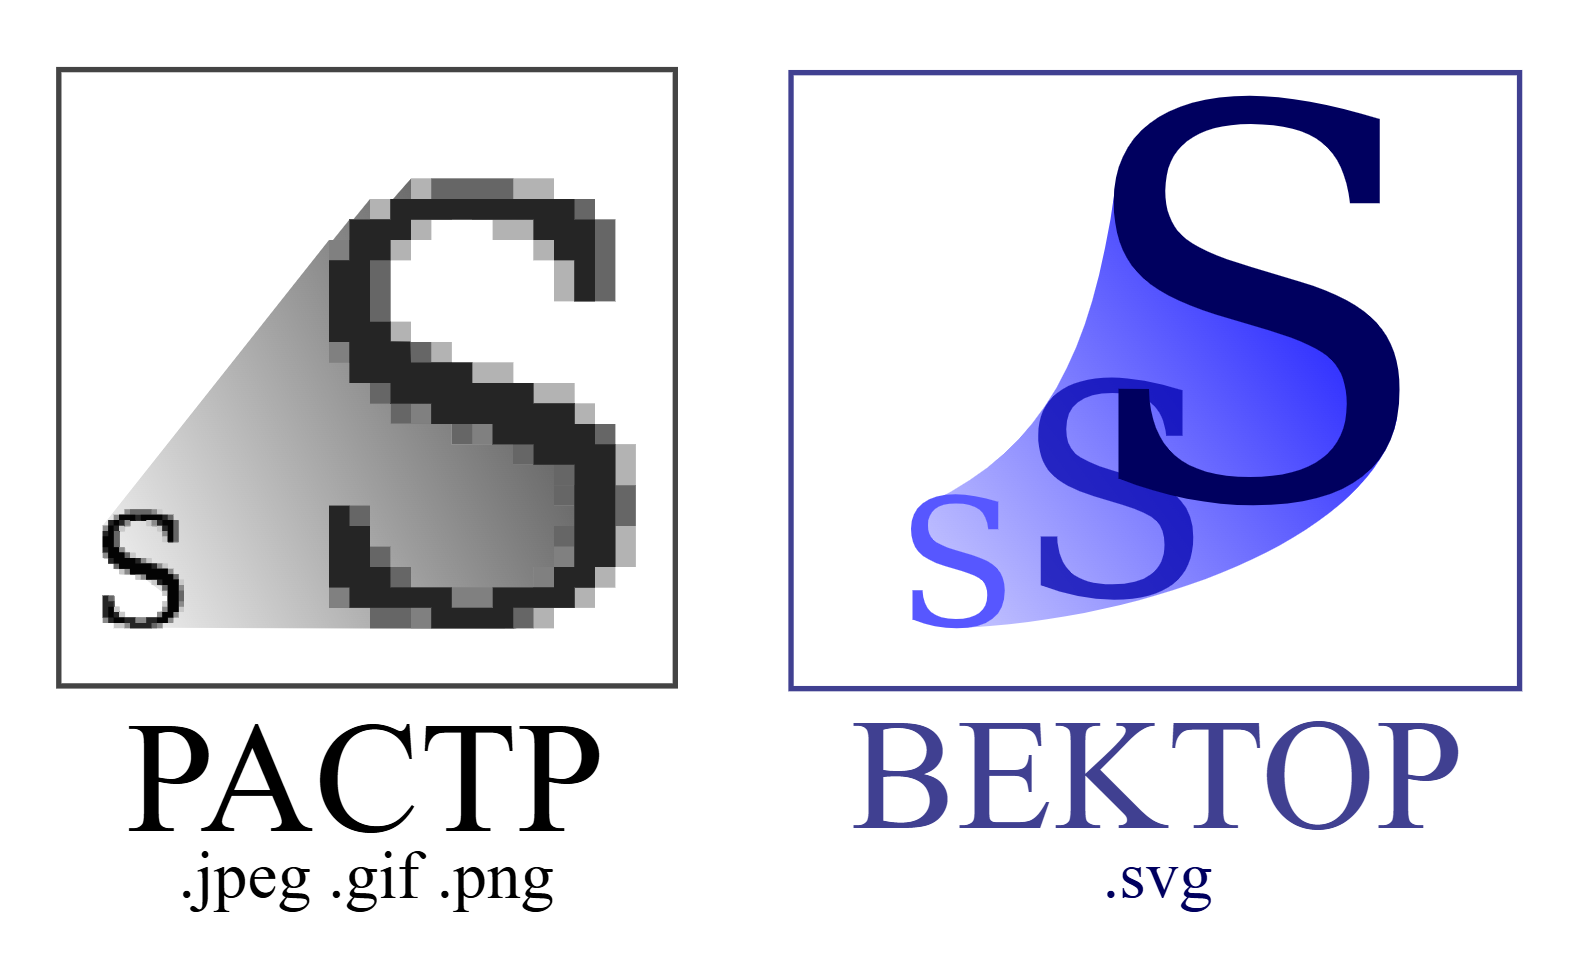
\includegraphics[width=0.8\textwidth]{r_v.PNG}

\end{center}

\subsection{Растровые представления изображений}
\label{base-section}
Растр~--- это общее двумерное графическое представление.
Растровое изображение~--- это цифровое изображение, представленное в виде двумерной сетки (матрицы) пикселей, где каждый пиксель характеризуется определённым цветом и интенсивностью.
\begin{center}
    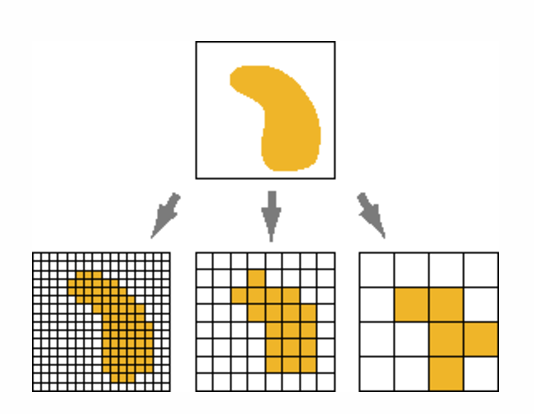
\includegraphics[width=0.8\textwidth]{rastr.png}

\end{center}
\paragraph{Вариации растров с геометрической точки зрения:}
\begin{enumerate}
    \item Двумерные (прямоугольные) растры (pixel)
    \item Шестиугольные (Рис.~\ref{ris:image1})
    \item Треугольные (Рис.~\ref{ris:image1})
    \item Неравномерные (Рис.~\ref{ris:image2})
    \item Трехмерные растры (voxel)
    \item Смешанные варианты (Рис.~\ref{ris:image3})
\end{enumerate}

\begin{figure}[H]
    \begin{center}
        \begin{minipage}[h]{0.4\linewidth}
            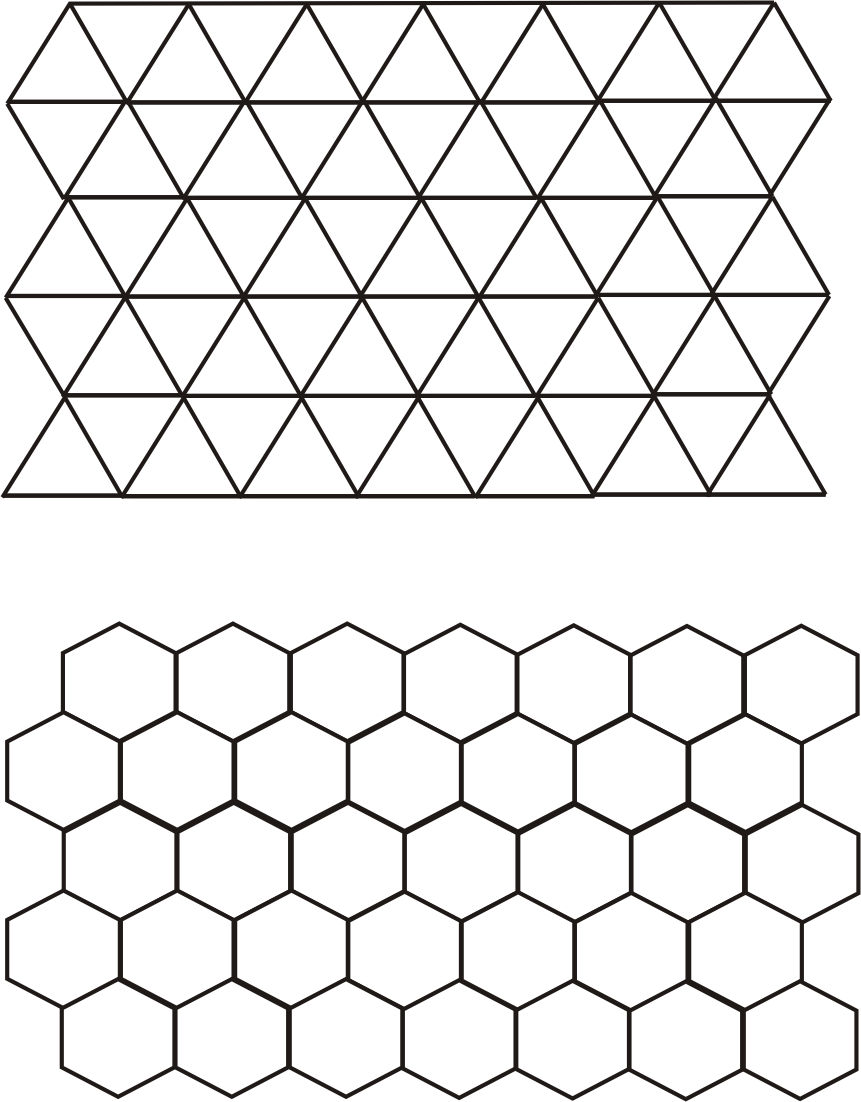
\includegraphics[width=1\linewidth]{r_tr_ge.png}
            \caption{Пример построения растров с треугольными и шестиугольными растровыми элементами.}
            \label{ris:image1}
        \end{minipage}
        \hfill
        \begin{minipage}[H]{0.4\linewidth}
            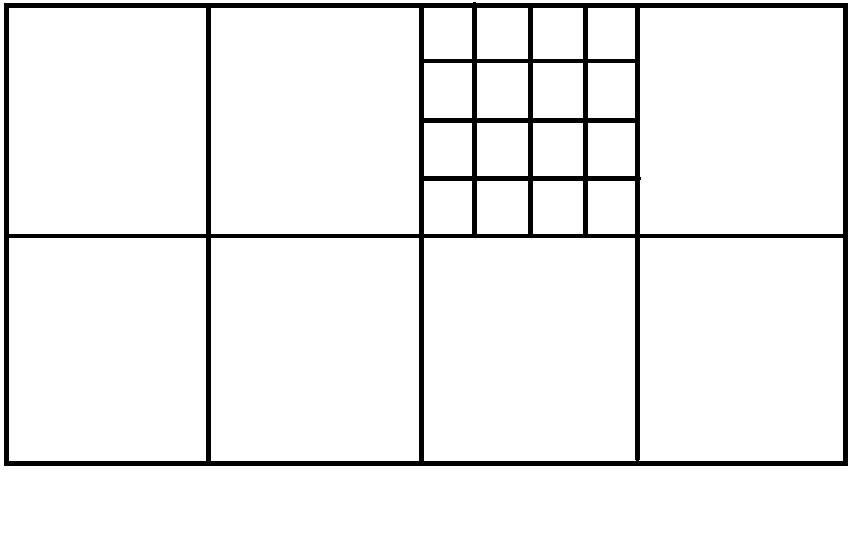
\includegraphics[width=1\textwidth]{r_ner1.png}
            \caption{Пример построения растров с неравномерными растровыми элементами.}
            \label{ris:image2}

            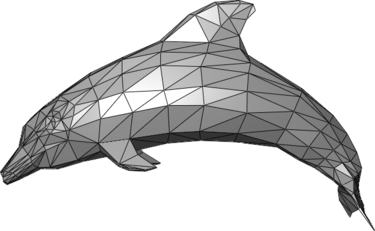
\includegraphics[width=1\textwidth]{mesh.png}
            \caption{Пример полигональной сетки (polygon mesh), изображающей дельфина.}
            \label{ris:image3}
        \end{minipage}
    \end{center}
\end{figure}

% \subsection{Особенности растровых изображений}
\subsubsection*{Недостатки}

\begin{enumerate}[label=\textbf{\arabic*.}, leftmargin=1.5em]

    \item \textbf{Ограниченное качество (отсутствие гладкости).}
          Растровые изображения не являются гладкими ни с точки зрения цветов, ни с точки зрения форм.
          \begin{itemize}
              \item Для устранения этих недостатков применяются алгоритмы сглаживания, однако они требуют значительных вычислительных ресурсов.
              \item Использование таких алгоритмов часто приводит к потере четкости из-за эффекта «размывания» изображения.
          \end{itemize}

    \item \textbf{Объем данных.}
          Объем памяти, занимаемый растровым изображением, пропорционален количеству ячеек в растре.
          \begin{itemize}
              \item Для передачи даже простых объектов требуется большое количество пикселей, что увеличивает требования к памяти и пропускной способности.
          \end{itemize}

    \item \textbf{Сложность проекции.}
          Для визуализации объектов в растровом формате необходимо выполнить их проекцию на растр.
          \begin{itemize}
              \item Проекция является вычислительно сложной операцией, особенно для трехмерных объектов.
          \end{itemize}

\end{enumerate}

\subsubsection*{Преимущества}
% \section*{Преимущества растровых изображений}

\begin{enumerate}[label=\textbf{\arabic*.}, leftmargin=1.5em]

    \item \textbf{Простота представления.}
          Растровые изображения хранятся в виде двумерного массива пикселей, где каждый пиксель характеризуется цветовым значением. Это упрощает их использование в цифровых устройствах и приложениях.

    \item \textbf{Простота отображения.}
          Растровый формат идеально подходит для вывода изображений на устройства визуализации, такие как мониторы и телевизоры. Представление пикселей напрямую соответствует структуре экрана, что делает отображение быстрым и эффективным.

    \item \textbf{Простота масштабирования.}
          \begin{itemize}
              \item \textit{Уменьшение:} Для уменьшения изображения достаточно выбирать отдельные пиксели или усреднять их значения в небольших областях (например, \(2 \times 2\)). Это позволяет создать уменьшенную версию изображения без сложных вычислений.
              \item \textit{Увеличение:} Изображение можно масштабировать до определенного предела, однако это может сопровождаться потерей качества из-за размытия или пикселизации.
          \end{itemize}

    \item \textbf{Алгоритмы на основе матричных преобразований.}
          В растровых изображениях алгоритмы обработки данных (например, фильтрация, вращение или масштабирование) могут быть представлены в виде матричных операций.
          \begin{itemize}
              \item \textit{Преимущества:}
                    \begin{itemize}
                        \item Легкость реализации таких алгоритмов в программном обеспечении.
                        \item Возможность аппаратного ускорения с использованием графических процессоров (GPU).
                        \item Высокая производительность при обработке больших объемов данных благодаря матричной структуре.
                    \end{itemize}
          \end{itemize}

\end{enumerate}

\subsection{Векторные представления изображений}
\label{base-section}
Векторное изображение~--- это цифровое графическое представление, в котором изображение формируется на основе математического описания примитивов, таких как линии, кривые, многоугольники и точки. Каждый элемент определяется параметрами, включая координаты, размеры, форму, цвет и другие атрибуты. %(Векторное изображение - список векторных объектов)
% \vspace{5mm}

\subsubsection*{Виды векторных представлений}

\begin{enumerate}[label=\textbf{\arabic*.}, leftmargin=1.5em]

    \item \textbf{Геометрические примитивы.}
          Простейшие элементы векторного представления, включающие прямые линии, кривые, окружности, многоугольники и точки.

    \item \textbf{Аппроксимация над примитивами.}
          \begin{itemize}
              \item При аппроксимации используется набор точек, а промежутки между ними описываются полиномами степени \( k \).
              \item \textit{Простейший случай:} кусочно-линейное приближение (\( k = 1 \)).
              \item \textit{Для \( k > 1 \):} существует бесконечное множество полиномов, но выбор можно ограничить условиями на гладкость (согласование производных первого, второго или более высоких порядков на границах участков).
              \item \textbf{Сплайны.} Если аппроксимация выполняется сплайнами степени \( k \), то на границах участков согласовываются условия на гладкость. Различные сплайны, такие как синусоидальные, обеспечивают гладкость, но не всегда дают визуально привлекательные результаты.
              \item \textbf{Альтернатива.} Для получения более простой аппроксимации можно использовать регрессионный подход:
                    \begin{itemize}
                        \item Прямая регрессия — построение одной прямой, которая с заданной точностью приближает набор точек.
                        \item Полиномиальная регрессия — выбор полинома определенной степени для лучшего приближения точек.

                              \begin{figure}[H]
                                  \begin{center}
                                      \begin{minipage}[h]{0.4\linewidth}
                                          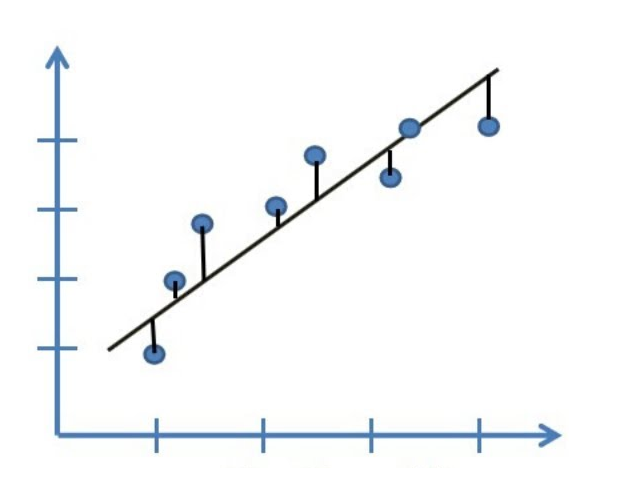
\includegraphics[width=1\textwidth]{line.png}
                                          \caption{Прямая регрессия.}
                                          \label{ris:arc}
                                      \end{minipage}
                                      \hfill
                                      \begin{minipage}[H]{0.4\linewidth}
                                          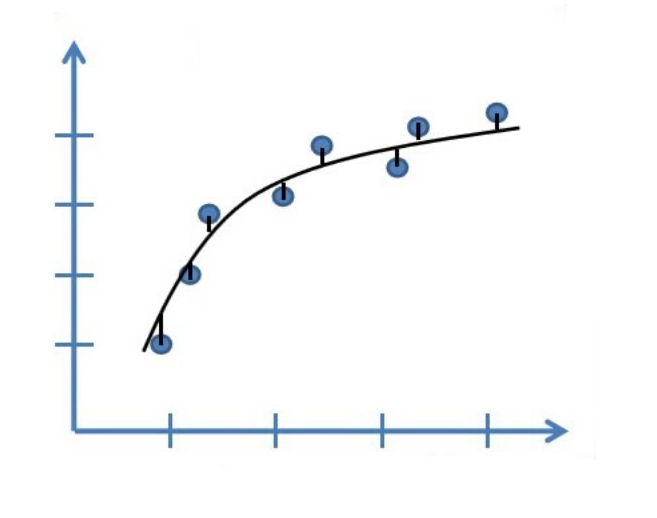
\includegraphics[width=1\textwidth]{poly.png}
                                          \caption{Полиномиальная регрессия.}
                                          \label{ris:arc}
                                      \end{minipage}
                                  \end{center}
                              \end{figure}

                    \end{itemize}
              \item \textbf{Недостатки регрессии:}
                    \begin{itemize}
                        \item Сложность контроля над формой кривой.
                        \item Ограниченное приближение сложных форм.
                        \item Часто не соответствует реальным изображениям.
                    \end{itemize}
                    % Решение этих проблем пришло из области автомобильного проектирования, а именно с кривыми Безье.
          \end{itemize}

    \item \textbf{Кривые Безье.}
          \begin{itemize}
              \item \textbf{Требования:}
                    Кривая должна соединять заданные точки \( P_0, P_1, \dots, P_n \), где каждая точка \( P_i \) задается набором координат:
                    \[
                        P_i = (x_1^i, x_2^i, \dots, x_k^i),
                    \]
                    где \( j \) — номер координаты, а \( i \) — индекс точки.

              \item \textbf{Параметрическое задание кривой:}
                    Кривая Безье определяется векторной функцией:
                    \[
                        B(t) = (Z^1(t), Z^2(t), \dots, Z^k(t)),
                    \]
                    где каждая координатная функция \( Z^j(t) \) имеет вид:
                    \[
                        Z^j(t) = \sum_{k=0}^n x_k^j \cdot b_{k,n}(t).
                    \]

              \item \textbf{Полиномы Бернштейна:}
                    \[
                        b_{k,n}(t) = C_n^k \cdot t^k (1-t)^{n-k},
                    \]
                    где \( C_n^k \) — биномиальный коэффициент.

          \end{itemize}

\end{enumerate}

\newpage

% Что даст такое задание кривой?
\paragraph{Примеры кривых для различных \textit{n}}
% \begin{center}
\subsubsection*{\textit{n} = 1}
% \end{center}
\begin{figure}[H]
    \begin{center}
        \begin{minipage}[h]{0.4\linewidth}
            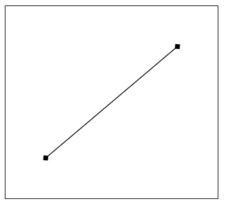
\includegraphics[width=1\linewidth]{TrueType_1_Line.PNG}
            \caption{Линейная кривая Безье.}
            \label{ris:line}
        \end{minipage}
    \end{center}
\end{figure}
Для \(n = 1\) кривая задаётся уравнением:
\[
    B(t) = (1-t)P_0 + tP_1.
\]
Это описывает отрезок,  опорные точки \(P_0\) и \(P_1\) определяют его начало и конец.
% \begin{center}
\subsubsection*{\textit{n} = 2}
% \end{center}

\begin{figure}[H]
    \begin{center}
        \begin{minipage}[h]{0.4\linewidth}
            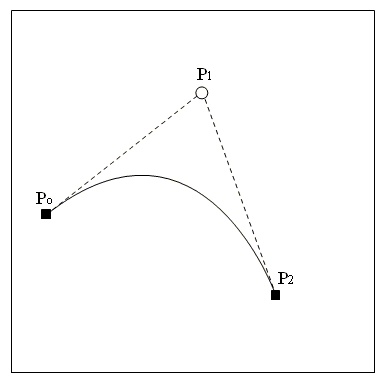
\includegraphics[width=1\textwidth]{TrueType_2_Arc.png}
            \caption{Квадратичная кривая Безье.}
            \label{ris:arc}
        \end{minipage}
    \end{center}
\end{figure}

Для \(n = 2\) кривая Безье имеет вид:
\[
    B(t) = (1-t)^2 P_0 + 2t(1-t)P_1 + t^2 P_2.
\]
Здесь \(2t(1-t)\) задает вершину параболы, проходящей через точки \(P_0\) и \(P_2\).
% \begin{center}
\subsubsection*{\textit{n} = 3}
% \end{center}

\begin{figure}[H]
    \begin{center}
        \begin{minipage}[h]{0.4\linewidth}
            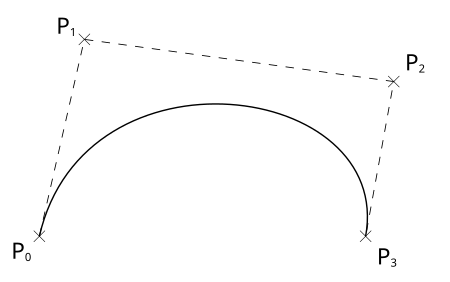
\includegraphics[width=1\textwidth]{Bezier_curve.png}
            \caption{Кубическая кривая Безье.}
            \label{ris:curve}
        \end{minipage}
    \end{center}
\end{figure}

Для \(n = 3\) формула становится:
\[
    B(t) = (1-t)^3 P_0 + 3t(1-t)^2  P_1 + 3t^2(1-t) P_2 + t^3 P_3.
\]
